\section{Material} % (fold)
\label{sec:material}
    \subsection{\aclp{TP}} % (fold)
        \label{sub:mapman}
        Für die Entwicklung von \protfin\ wurden 41669 MapMan-Referenz-Pflanzenproteine verwendet (\texttt{protein.fa} im \Anhang), die dem Trainieren von Bin-spezifischen Hidden Markov Models von MapMan4 dienten \autocite{mapman}, siehe \Anhang. MapMan ist eine für Pflanzen entwickelte Methode, um deren Proteinsequenzen in diesen Bins nach Funktion zu klassifizieren. Dies erfolgt in einer Baumstruktur, wobei die Wurzelknoten sowie die Knoten je Ebene eines Baums von 1 aufsteigend nummeriert sind. Die Wurzelknoten sind grobe Beschreibungen der Funktion, wie zum Beispiel der Photosynthese. Je mehr der Baum in die Tiefe geht, desto präziser wird die Beschreibung, bis an den Blättern die Proteine mit ihrer Annotation stehen \autocite{mapman}\autocite{mapman}. Ein Bin setzt sich aus der Konkatenation seiner Knoten mittels Punkt als Separator zusammen. So ist in \texttt{mapman.tsv} im \Anhang\ zum Beispiel der Bin 1.1.1, wobei die linke Ziffer für die Wurzel Photosynthese steht, die mittlere Ziffer für die Photophosphorylation und die dritte für das betreffende Photosystem 2. Aufgrund dieser Klassifizierung nach Funktion werden die Bins der Proteine in \protfin\ als Familien betrachtet und gehen daher in die Bewertung der Identifikation von Funktionsgleichheit ein.

        \begin{figure}[H]
            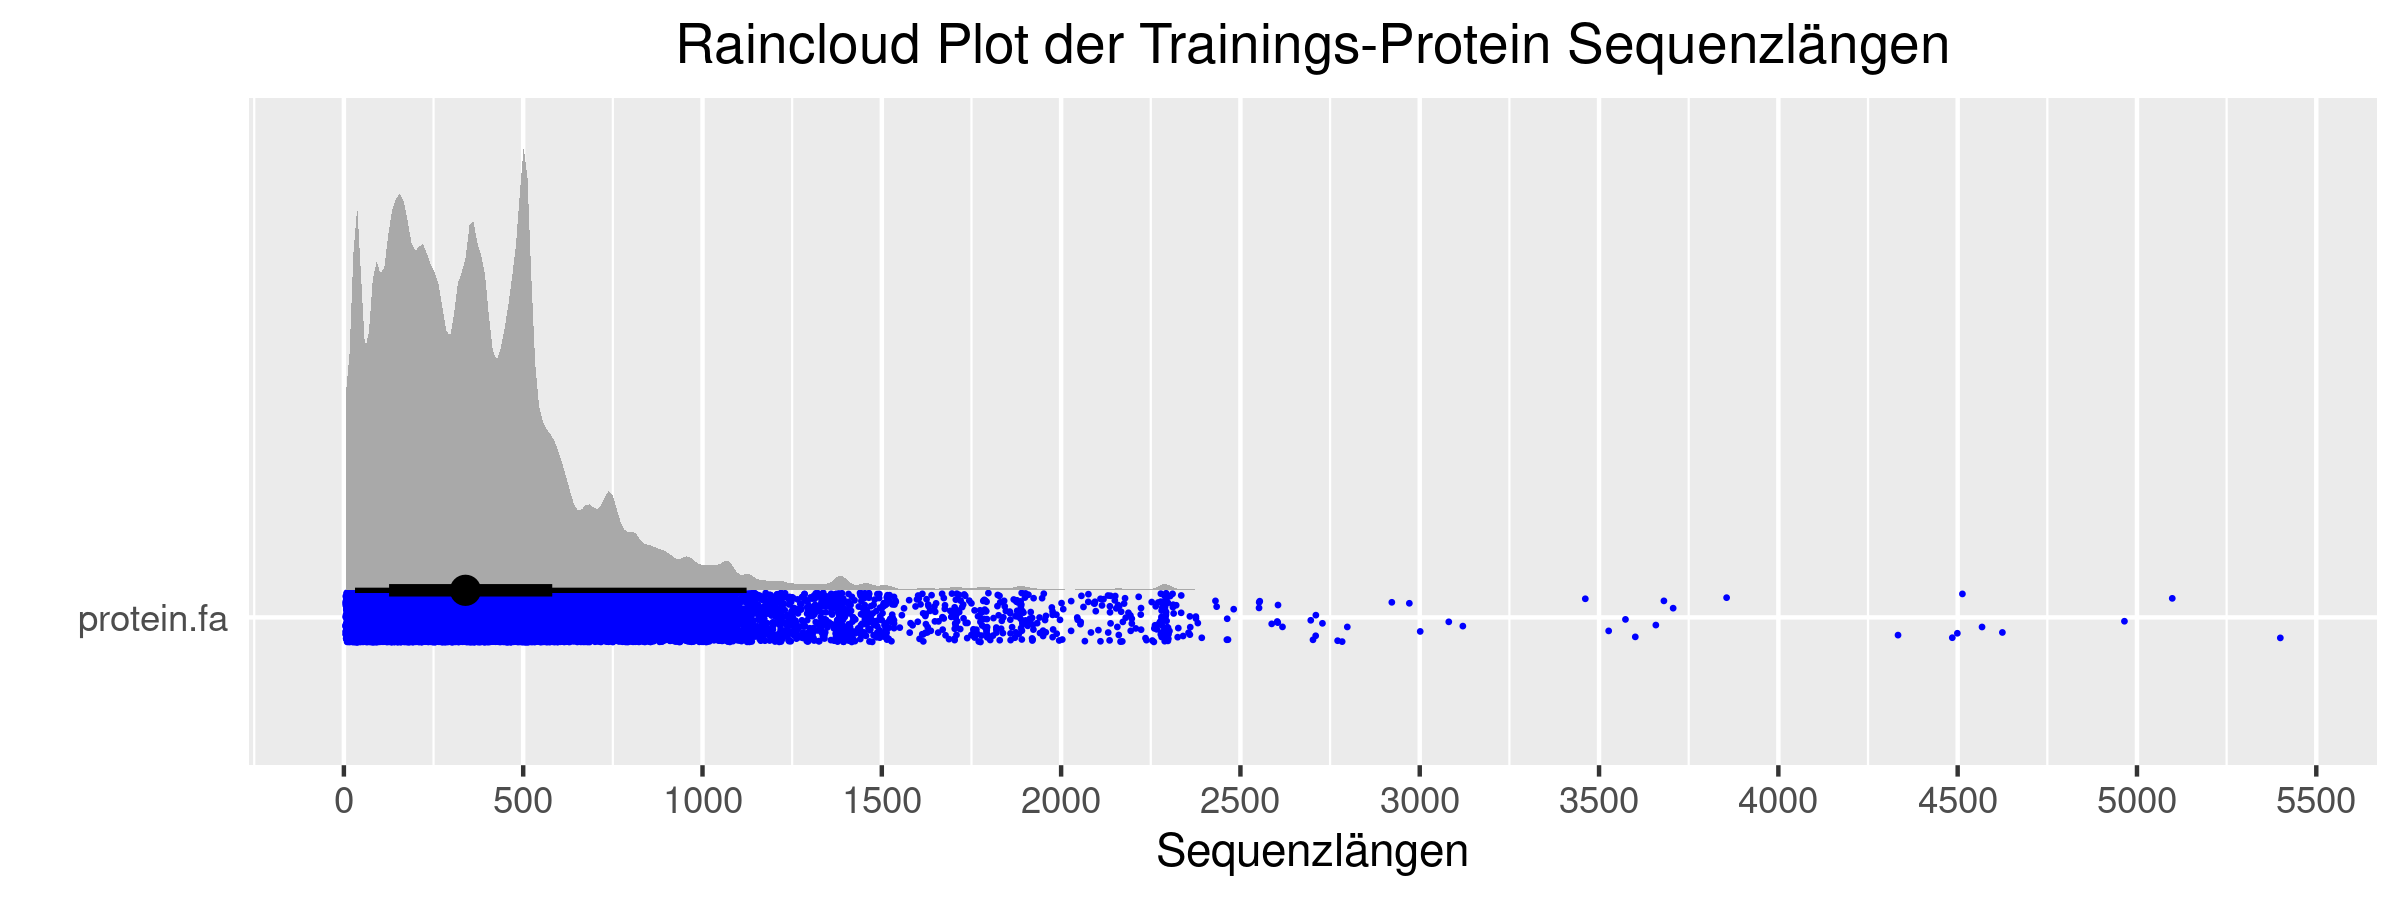
\includegraphics[width=\textwidth]{seq_lens.png}
            \caption[Raincloud Plot der \acl Sequenzlängen]{Die graue ``Wolke'' des Raincloud Plots stellt die Dichteverteilung der Sequenzlängen über die 41669 MapMan-Referenz-Proteine (\acl{TP}) dar, die blauen Punkte darunter, welche Werte tatsächlich angenommen wurden, und dazwischen ist ein Boxplot, der Aufschluss über den Median (schwarzer Kreis) und die anderen Quartile bietet. Die mediale Länge liegt bei etwa 300 Aminosäuren.}
            \label{fig:sequences}
        \end{figure}

    % subsection ac (end)
    \subsection{UniRef90} % (fold)
        \label{sub:uniref90}
        In der UniRef90-Datenbank sind Sequenzen aus der UniProtKB \autocite{uniprot} mit 90\% Sequenzübereinstimmung in sogenannten UniRef-Einträgen gruppiert, welche verschiedenste Informationen über die Gruppe bieten. Zudem ist jedem Eintrag die Proteinsequenz zugeordnet, die die Gruppe am besten repräsentiert \autocite{uniref}. UniRef-Datenbanken werden regelmäßig erneuert. Für die Experimente in \protfin\ mit der UniRef90-Datenbank wird der Release 2024\_02 (27.03.2024) verwendet:

        \href{https://ftp.uniprot.org/pub/databases/uniprot/previous_releases/release-2024_02/}{\centerIt{\text{https://ftp.uniprot.org/pub/databases/uniprot/previous\_releases/release-2024\_02/}}}

        Die entpackte FASTA-Datei ist etwa 82 Gigabyte groß und enthält 187.136.236 Proteinsequenzen. Sie befindet sich zum Zeitpunkt der Abgabe dieser Arbeit auf dem Compute Cluster der Hochschule an folgendem Pfad:

        \centerIt{\texttt{/media/BioNAS/UniProtKB/20240408/uniref90.fasta}}
    % subsection uniref90 (end)
% section material (end)

\section{Methoden} % (fold)
    \label{sec:methoden}
    % Erhalt numerischer Vektoren
    Jeglicher Code, ob für die konkrete Implementierung der Algorithmen oder der durchgeführten Experimente, wurde mit versioniert und ist auf GitHub verfügbar. Die genauen Verweise, was wo hinterlegt ist, sind im \Anhang\ zu finden.

    \subsection{Grundalgorithmus} % (fold)
        \label{sub:grundalgorithmus}
        \begin{algorithm}[H]
            \caption{Übersetzen einer Aminosäuresequenz in einen numerischen Vektor}\label{alg:vorbereitung}
            \PhantomSubSub{Übersetzen einer Aminosäuresequenz in einen numerischen Vektor}
            Eingabe sind eine Aminosäuresequenz und die Nummer eines \acl{KF}s, beginnend mit 0. Dann wird die Sequenz zeichenweise in einen Vektor übersetzt, wobei erst der Wert des \ac{KF} abgerufen wird und dieser dann auf einen positiven Wert normalisiert wird.
            \newcommand{\I}{\text{\textquotesingle}}
            \begin{algorithmic}[1]

                \myRequire{
                    $sequence \in \{ \text{A-Z}, \I\Psi\I, \I\Omega\I, \I\Phi\I, \I\zeta\I, \I\Pi\I, \I\text{+}\I, \I\text{-}\I\}^{*} $\\
                    $0 \leq kf \leq 9$
                }
                \myEnsure{
                    $|aa\_vector| = |sequence|$ \Comment $aa = \emph{Aminosäure}$\\
                    $v \geq 0\ \forall\ v \in aa\_vector$
                }

                \State $aa\_vector \gets \texttt{array}()$
                \ForEach{$aa$}{$sequence$}
                    \State $kf\_value \gets \texttt{get\_kf\_value}(aa, kf)$ \Comment $kf=Kidera\ Faktor$
                    \State $min\_kf\_value \gets \texttt{get\_min\_kf\_value}()$
                    \State $aa\_vector.\texttt{append}(kf\_value + \texttt{abs}(min\_kf\_value))$
                \EndFor
            \end{algorithmic}
        \end{algorithm}
        Voraussetzung für den Algorithmus ist ein numerischer Vektor, so wie es die digitale Tonspur bei SHAZAM darstellt. Um dies im Kontext von Proteinen zu erreichen, wird in \protfin\ auf sogenannte Kidera-Faktoren zurückgegriffen. Diese Faktoren stammen aus einem Forschungsprojekt von \citeauthor{kidera}, welches \citefield{kidera}{year} publiziert wurde \autocite{kidera}. Inhalt des Projekts war die statistische Faktorenanalyse von 188 physikalischen Eigenschaften der 20 natürlichen Aminosäuren zur Ermittlung von 10 dieser Eigenschaften, durch die die anderen aufgrund hoher Korrelation erklärt werden können. Dadurch, dass die wenigen \ac{KF} all die Eigenschaften repräsentieren, können diese effizient gleichzeitig analysiert werden. In \autoref{tab:kidera} sind die \ac{KF} dargestellt.

        \begin{table}[H]
            \hfill\caption[Kidera-Faktoren]{Kidera-Faktoren}
            \label{tab:kidera}
            \begin{minipage}{\textwidth}
                Jeder Kidera-Faktor hat eine eigene Zeile mit seiner beschreibenden Bezeichnung in der linken Spalte, danach folgen die Werte je Aminosäure. Die vollständige Tabelle ist im \Anhang\ in \texttt{Amino\_Acid\_Kidera\_Factors.csv} zu finden und stammt aus dem R-Paket ``Peptides'' \autocite{peptides}.
            \end{minipage}
            \newcommand{\T}[1]{\centerIt{\textbf{#1}}}
            \centerIt{
            \csvreader[tabular=lllllllll,
              table head=\toprule\T{Beschreibung} & \T{A} & \T{C} & \T{D} & \T{E} & \T{F} & \T{G} & \textbf{\dots}\\\midrule,
              head to column names,
              late after line=\\,
              late after last line=\\\bottomrule
              ]%
              {../CD/Supplement/material/Amino_Acid_Kidera_Factors.csv}{Kidera_Factor=\KF, Kidera_Factor_Description=\KFD}%
            {\KFD & \A  & \C & \D & \E & \F & \G & \dots}}
        \end{table}

        Folglich kann eine Aminosäuresequenz pro \ac{KF} in einen numerischen Vektor übersetzt werden, wobei ein höherer absoluter Wert für mehr Relevanz des \ac{KF} steht.

        Um für die Fourier Transformation nur positive Werte zu verwenden, wird der Vektor anschließend dahingehend normalisiert, dass das absolute Minimum aller Werte aus \autoref{tab:kidera} aufaddiert wird. Das absolute Minimum ist 2.33, sodass die Übersetzung der Beispielsequenz \texttt{EVKEFDGQGCFC} für die Hydrophobizität folgendermaßen geschehe:

        \begin{figure}[H]
            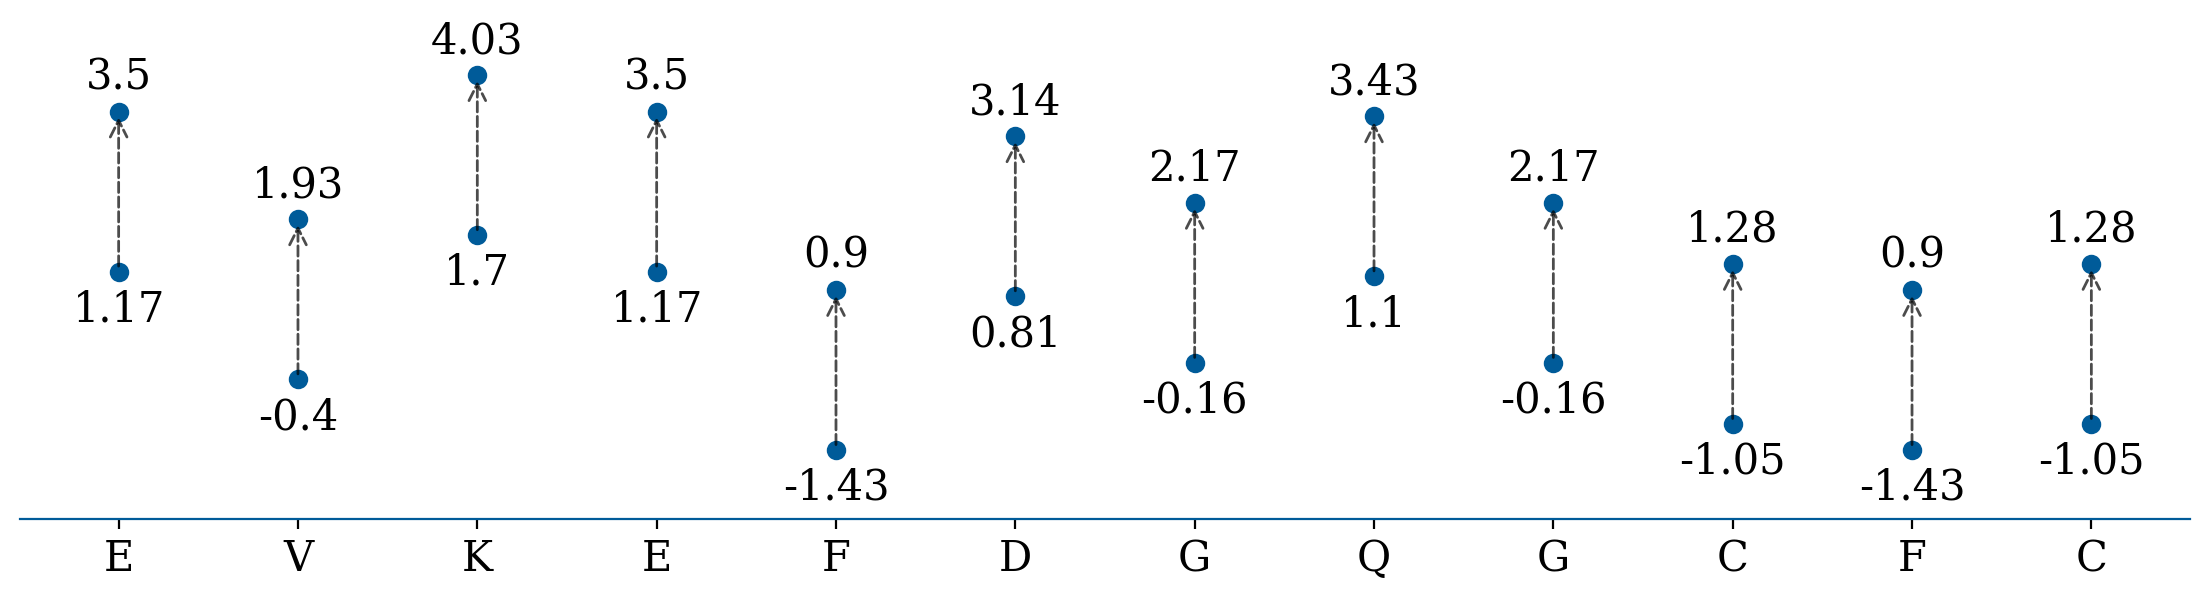
\includegraphics[width=\textwidth]{aa_vec.png}
            \caption[Beispielsequenz als numerische Repräsentation]{Beispielsequenz als numerische Repräsentation: Je Aminosäure auf der x-Achse entspricht der untere Punkt ihrem Wert für ``Hydrophobicity'' aus \autoref{tab:kidera}. Der Pfeil symbolisiert die Normalisierung dieses Wertes durch das Inkrement von 2.33. Die horizontale Linie ist die Nulllinie.}
            \label{fig:normalization}
        \end{figure}

        % Sammeln struktureller Information
        % \vspace{2.25mm}
        \begin{algorithm}[H]
            \caption{Sammeln von Strukturdaten}\label{alg:strukturdaten}
            \PhantomSubSub{Sammeln von Strukturdaten}
            Eingabe ist der Vektor aus \autoref{alg:vorbereitung}. Dieser wird mittels \acs{STFT} fensterweise transformiert und anschließend je Fenster die Frequenzen ausgewählt, deren Amplituden ein lokales Maximum bilden, und zur \acl{CM} hinzugefügt.
            \begin{algorithmic}[1]
                \Require $aa\_vector$ aus \autoref{alg:vorbereitung} \Comment $aa = \emph{Aminosäure}$
                \Ensure $constellation\_map$ is an Array of Arrays of Floats

                \State $constellation\_map \gets \texttt{array}()$
                \State $stft\_result \gets \texttt{stft\_transform}(aa\_vector)$\AlgLineLabel{alg:strukturdaten:stft}
                \ForEach{$window$}{$stft\_result$}
                    \State $selected\_frequencies \gets \texttt{select\_maxima}(window)$\AlgLineLabel{alg:strukturdaten:selection}
                    \State $constellation\_map.\texttt{append}(selected\_frequencies)$
                \EndFor
            \end{algorithmic}
        \end{algorithm}
        Der erhaltene Vektor aus \autoref{alg:vorbereitung} wird strukturell analysiert. Das dafür genutzte Vorgehen basiert auf der \ac{STFT}, welche den Vektor fensterweise auf periodische Signale untersucht, wie z.B. dem wiederholten Auftreten von hydrophoben Aminosäuren im gleichen Abstand oder in der Musik ein Refrain oder dem Rhythmus. Für die \ac{STFT} in \protfin\ Version 0.4 wird die Methode \texttt{stft} aus dem Untermodul \texttt{signal} des Python-Moduls \texttt{scipy} \autoref{scipy} Version 1.11.4 verwendet. Je Fenster werden die Frequenzen der auffälligsten Signale ausgewählt, wie in \autoref{fig:freq_selection} dargestellt mittels der lokalen Maxima, sodass über alle Intervalle eine sogenannte Constellation-Map entsteht, welche in der folgenden \autoref{fig:hashing} im linken Teil dargestellt ist. Diese Map wird dabei als Array repräsentiert, wobei jedes Element hierbei eine Liste darstellt, die ihrem Index entsprechend die gewählten Frequenzen des jeweiligen Fensters beinhaltet.

        \begin{figure}[H]
            \centering
            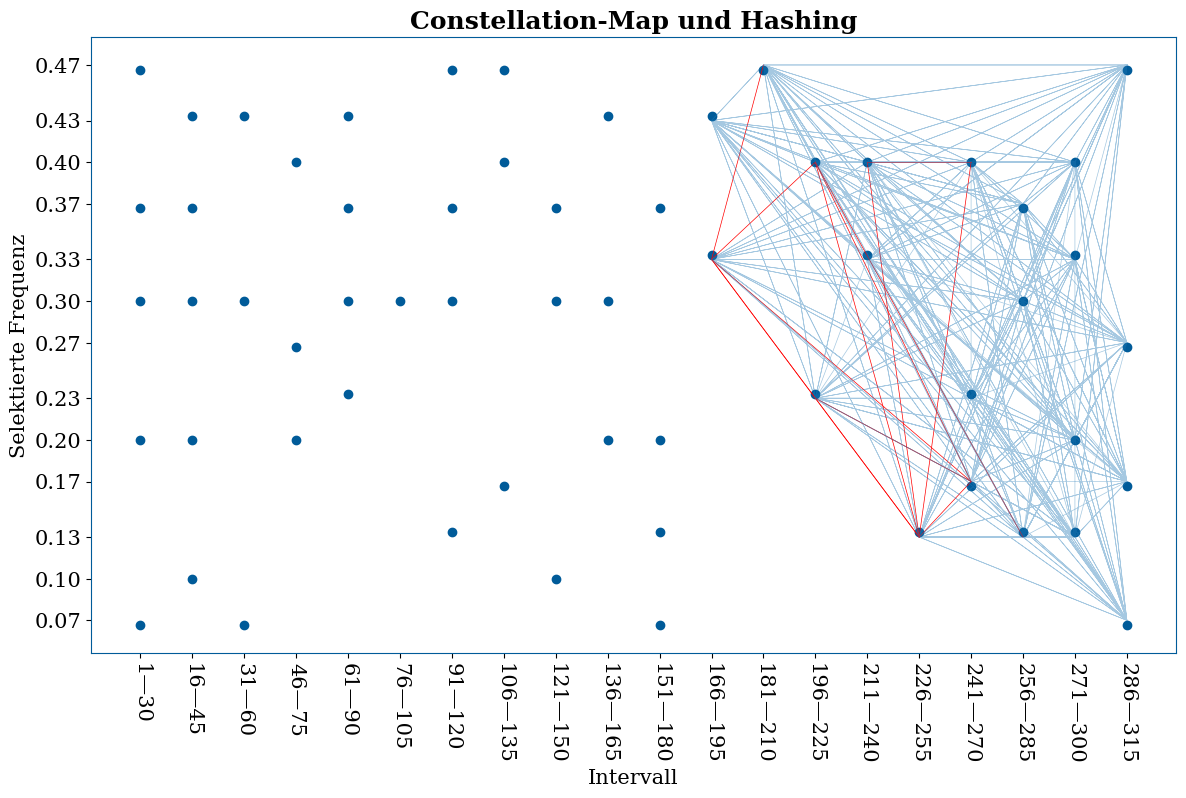
\includegraphics[width=1\textwidth]{plot_method.png}
            \caption[Constellation-Map und Hashing]{Die Punkte bilden die Constellation-Map. Auf der y-Achse ist die Frequenz und auf der x-Achse das Intervall des STFT-Fensters. Die zur Übersicht nur rechts eingezeichneten Kanten repräsentieren die Hash-Bildung aus dieser Constellation-Map, wobei rote Kanten ignorierte Hashes darstellen, weil sie in einem Nachfolgefenster erneut auftauchen und nur das letzte Vorkommen gespeichert wird.}
            \label{fig:hashing}
        \end{figure}

        % Hashing
        % \vspace{2.25mm}
        \begin{algorithm}[H]
            \caption{Hashing}\label{alg:hashing}
            \PhantomSubSub{Hashing}
            Eingabe ist eine \acl{CM} aus \autoref{alg:strukturdaten}, die ID des betreffenden Proteins und die Nummer des \acl{KF}s, beginnend bei 0. Je Fenster wird jede Frequenz A paarweise mit den Frequenzen aus allen Nachfolgefenstern kombiniert. Die Frequenz A, die jeweilige Nachfolgefrequenz, der Abstand zur Nachfolgefrequenz und die Nummer des \acl{KF}s bilden den Hash. Der Abstand darf 12 Bit, also $2^{12}$ nicht überschreiten, siehe nachfolgende \label{fig:hash}. Je Hash wird die Position des Fensters von Frequenz A in der \acl{CM} gespeichert und zusätzlich die Protein-ID, um die Verbindung von Hash und Protein zu erhalten.
            \begin{algorithmic}[1]
                \myRequire{
                    $constellation\_map$ aus \autoref{alg:strukturdaten}\\
                    $protein\_id$ is a String\\
                    $0 \leq kf \leq 10$
                }
                \Ensure $hashes$ is a HashMap of: $Int \rightarrow Int, String$

                \State $hashes \gets \texttt{hashmap}()$
                \State $window\_idx \gets 0$
                \Repeat
                    \State $selected\_frequencies \gets constellation\_map.\texttt{pop}(0)$
                    \ForEach{$frequency$}{$selected\_frequencies$}
                        \State $successor\_count \gets \texttt{min}(2^{12}, \texttt{length}(constellation\_map)) - 1$\AlgLineLabel{alg:hashing:target_zone}
                        \For{$successor\_idx \gets 0\ \textbf{to}\ successor\_count$}
                            \State $succ\_frequencies \gets constellation\_map[successor\_idx]$
                            \ForEach{$succ\_frequency$}{$succ\_frequencies$}
                                \State $hash \gets \texttt{create\_hash}(frequency, succ\_frequency, successor\_idx, kf)$
                                \State $hashes[hash] \gets (window\_idx, protein\_id)$
                            \EndFor
                        \EndFor
                    \EndFor
                    \State $window\_idx \gets window\_idx + 1$
                \Until{$constellation\_map$ is empty}
            \end{algorithmic}
        \end{algorithm}

        Die erhaltene \ac{CM} wird elementweise gehashed, um einen effizienten Vergleich mit anderen \ac{CM}s zu ermöglichen. Um das zu erzielen, wird jede ausgewählte Frequenz eines Fensters mit jeder weiteren Frequenz der Nachfolgefenster gepaart. Bildlich gesprochen werden also Kanten gebildet, wodurch die \ac{CM} zu einem Graphen wird. Jede dieser Kanten bildet einen Hash, also einer Kombination aus den beiden Frequenzen/Kantenenden und der Kantenlänge (hier $\texttt{successor\_idx}$, beginnend mit 0). In einer HashMap (für \protfin\ Version 0.4 in Python ein Dictionary) wird sich folgend für den Hash die Position der Kante in der \ac{CM} gemerkt, sowie die ID des Proteins, für die diese \ac{CM} erstellt wurde. Sollte ein Hash dabei mehrfach vorkommen, verbleibt lediglich seine letzte Position. Dieses Verfahren wird im rechten Teil von \autoref{fig:hashing} repräsentativ dargestellt, wobei rote Linien die ignorierten Kanten abbilden.


        \newpage
        Die Hashfunktion ist bijektiv gestaltet, sodass aus einem Hash all seine Bestandteile, die für die Erstellung verwendet wurden, eindeutig abgeleitet werden können. Das hängt damit zusammen, dass diese Bestandteile nach folgendem Schema auf Bit-Ebene hintereinandergereiht werden:

        \begin{figure}[H]
            \newcommand{\Col}[2]{\multicolumn{1}{|@{}p{#1\linewidth}@{}|}{\centering #2}}
            \centering
            \begin{tabular}{@{}p{0.1875\linewidth}@{}p{0.125\linewidth}@{}p{0.375\linewidth}@{}p{0.15625\linewidth}@{}p{0.15625\linewidth}@{}}
            % \begin{tabular}{|@{}p{0.125\linewidth}@{}|@{}p{0.375\linewidth}@{}|@{}p{0.15625\linewidth}@{}|@{}p{0.15625\linewidth}@{}|}
                \hline
                \Col{0.1875}{6 Bit} & \Col{0.125}{ 4 Bit} & \Col{0.375}{12 Bit} & \Col{0.15625}{5 Bit} & \Col{0.15625}{5 Bit}\\
                \hline
                \centering \textit{unbelegt} & \centering \acl{KF} & \centering Kantenlänge/Fensterabstand & \centering Frequenz Nachfolger & \centering Frequenz Ursprung
                % 4 Bit & 18 Bit & 5 Bit & 5 Bit\\
            \end{tabular}
            \caption[Schematischer Aufbau eines Hashes]{Schematischer Aufbau eines Hashes: 4 Bit werden für die Nummer eines \acl{KF}s belegt. Die Fenstergrößen belaufen sich auf unter 64, sodass mit 5 Bit alle möglichen Frequenzen abgedeckt werden können. Da die Anzahl Frequenzen immer gleich ist, können diese aufsteigend durchnummeriert werden, sodass die x-Achse in \autoref{fig:freq_selection} der Folge von 0 bis 15 entspräche. 12 Bit enthalten die ``Kantenlänge'' eines Hashes. Die restlichen 6 Bits zu einem 32-Bit Integer können in der weiteren Entwicklung des Algorithmus beliebig belegt werden.}
            \label{fig:hash}
        \end{figure}

        % Erstellung der Datenbank
        \begin{algorithm}[H]
            \caption{Erstellung der Datenbank}\label{alg:datenbank}
            \PhantomSubSub{Erstellung der Datenbank}
            Eingabe ist eine Datei im FASTA-Format. Aus jeder darin befindlichen Sequenz wird nach \autoref{alg:vorbereitung} ein numerischer Vektor erstellt, dieser dann mittels \autoref{alg:strukturdaten} in eine \acl{CM} übersetzt und diese anschließend dem \autoref{alg:hashing} entsprechend gehashed. Je Hash wird das Tupel aus Position, an der der Hash in der \acl{CM} auftauchte, und Protein-ID in eine Liste in der Datenbank eingefügt, auf die der Hash verweist.
            \begin{algorithmic}[1]
                \Require $fasta$ is a FASTA-formatted file
                \Ensure $database$ is a HashMap of: $Int \rightarrow Array\ of\ (Int, String)$

                \State $database \gets \texttt{hashmap}()$
                \ForEach{$protein\_id, sequence$}{$fasta$}
                    \For{$kf \gets 0\ \textbf{to}\ 10$} \Comment $kf=Kidera\ Faktor$
                        \State $aa\_vector \gets \texttt{get\_aa\_vector}(sequence, kf)$ \Comment $aa = \emph{Aminosäure}$
                        \State $constellation\_map \gets \texttt{get\_constellation\_map}(aa\_vector)$
                        \State $hashes \gets \texttt{get\_hashes}(constellation\_map, protein\_id)$
                        \ForEach{$hash$}{$hashes$}
                            \If{$hash\ \textbf{not in}\ database$}
                                \State $database[hash] \gets \texttt{array}()$
                            \EndIf
                            \State $database[hash].\texttt{append}(hashes[hash])$
                        \EndFor
                    \EndFor
                \EndFor
                \State $\texttt{save\_to\_file}(database)$
            \end{algorithmic}
        \end{algorithm}

        Die beschriebenen Algorithmen~\ref{alg:vorbereitung} bis~\ref{alg:hashing} beschreiben den Weg von einer Aminosäuresequenz in Textform zu den Hashes, die die strukturelle Information des Proteins entsprechend der spektralen Zerlegung mittels \ac{STFT} repräsentieren sollen. Übrig bleibt nur der Schritt, der die Hashes einer Menge von mehreren Proteinen in einer Datenbank vereinigt, sodass im Anschluss die Identifizierung von Eingabesequenzen erfolgen kann. Dafür werden je \ac{TP} für alle Kidera-Faktoren die Hashes gebildet und in die Datenbank geschrieben, welche eine HashMap ist. Im Gegensatz zu der resultierenden HashMap in \autoref{alg:hashing} verweisen die Hashes in der Datenbank allerdings nicht auf eine Position des Hashes für ein Protein, sondern auf eine Liste von solchen. Das heißt, dass für die Datenbank ein neuer Hash mit einem leeren Array initialisiert wird, in das darauf all diese Position-Protein-ID-Tupel eingefügt werden.

        Version 0.4 von \protfin\ ist in Python implementiert. Von daher wird für die Persistierung der Datenbank (\texttt{save\_to\_file}) zur Einfachheit das \texttt{pickle}-Modul verwendet, welches mit der genutzten Python-Version 3.10.12 mitgeliefert wird und Python-Objekte effizient in Dateien ablegen kann.

        % hierzu ein Plot zur Veranschaulichung der Offsets
        % Scoring/Map-Vergleich
        Wurde die Datenbank erstellt, ist sie für die Identifizierung funktionsähnlicher Proteine anhand einer Eingabe verwendbar. Hierfür gibt es zwei Ansätze:
        \begin{enumerate}[a)]
            \item \PhantomSubSub[sp.matching]{Single-Protein-Matching}
                \textbf{Single-Protein-Matching:}\ \ Eingabe ist eine FASTA-Datei, also eine Menge an Suchsequenzen. Ausgabe je Sequenz ist eine Liste von Treffern, sortiert nach Übereinstimmung der Hashes der Constellation-Maps von Treffer und Suchsequenz. Je höher der Rang eines Treffers, desto funktionsähnlicher sollte das entsprechende Protein sein. Treffer mit dem besten Score erhalten Rang 1, mit dem zweitbesten Score Rang 2, \dots und der Treffer mit dem schlechtesten Score den letzten Rang. Die Ausgabe in \protfin\ Version 0.4 sind \ac{CSV}, also eine durch Kommata separierte Tabelle, mit folgenden Spalteninhalten:
                \begin{enumerate}[1.]
                    \item Rank $\rightarrow$ Rang
                    \item Match\_Protein\_ID $\rightarrow$ Protein-ID des Treffers
                    \item JSI $\rightarrow$ Jaccard Similarity Index (siehe \autoref{alg:scoring})
                    \item Score $\rightarrow$ Score (Übereinstimmung der Constellation-Map)
                    \item Input\_Protein\_ID $\rightarrow$ Protein-ID der Suchsequenz
                    \item Input\_Sequence\_Length $\rightarrow$ Sequenzlänge der Suchsequenz
                    \item Input\_Found\_Hashes $\rightarrow$ Anzahl Hashes der Suchsequenz
                \end{enumerate}

                \newcommand{\Width}{\dimexpr\textwidth-\leftmargin}
                \begin{minipage}{\Width}
                    \begin{algorithm}[H]
                        \caption{Treffer-Bewertung beim Single-Protein-Matching}\label{alg:scoring}
                        Eingabe sind die Hashes für die Suchsequenz nach \autoref{alg:hashing} und die trainierte Datenbank aus \autoref{alg:datenbank}. Für jeden Hash der Suchsequenz S wird für jedes Protein P in der Datenbank mit diesem Hash der Abstand/Offset seiner Position in der \acf{CM} von der Position von P in dessen \acs{CM} gebildet. Für P wird gezählt, wie oft ein jeder Offset vorkommt. Der Score von P bildet sich durch die Anzahl des häufigsten Offsets und dem nachfolgend in \autoref{equ:jsi} beschriebenen \acl{JSI}.
                        \begin{algorithmic}[1]
                            \myRequire{
                                $hashes$ aus \autoref{alg:hashing}\\
                                $database$ aus \autoref{alg:datenbank}
                            }
                            \Ensure $match\_scores$ is a HashMap of: $String \rightarrow Float$

                            \State $matches\_per\_tp \gets \texttt{hashmap}()$ \Comment $tp=Trainings Protein$
                            \ForEach{$hash, position$}{$hashes$}
                                \If{$hash\ \textbf{in}\ database$}
                                    \ForEach{$tp\_position, protein\_id$}{$database[hash]$}
                                        \If{$protein\_id\ \textbf{not in}\ matches\_per\_tp$}
                                            \State $matches\_per\_tp[protein\_id] \gets \texttt{hashmap}()$
                                        \EndIf
                                        \State $offset \gets tp\_position - position$
                                        \If{$offset\ \textbf{not in}\ matches\_per\_tp[protein\_id]$}
                                            \State $matches\_per\_tp[protein\_id][offset] \gets 0$
                                        \EndIf
                                        \State $offset\_count \gets matches\_per\_tp[protein\_id][offset]$
                                        \State $matches\_per\_tp[protein\_id][offset] \gets offset\_count + 1$
                                    \EndFor
                                \EndIf
                            \EndFor
                            \State $match\_scores \gets \texttt{hashmap}()$
                            \ForEach{$protein, offsets$}{$matches\_per\_tp$}
                                \State $score \gets \texttt{get\_most\_common\_offset}(offsets)$
                                \State $match\_protein\_hashes \gets database.\texttt{get\_hashes}(protein)$
                                \State $jsi \gets \texttt{get\_jsi}(hashes, match\_protein\_hashes)$

                                \State $match\_scores[protein] \gets score \cdot jsi$
                            \EndFor
                        \end{algorithmic}
                    \end{algorithm}
                \end{minipage}\hfill\\\hfill\\

                Um den Score zu bestimmen, also die Ähnlichkeit der \ac{CM} der Eingabe mit denen der \ac{TP}, werden pro Eingabe-Hash die Differenzen zwischen dessen Position mit den Positionen der trainierten Hashes gebildet und global pro Protein gezählt. Diese Differenzen repräsentieren den Abstand/Offset der Kante in der Eingabe-Map zur Kante der jeweiligen \ac{TP}-Map, also wie weit die Eingabe-Map verschoben wäre, sollte es sich bei dem \ac{TP} um das Original handeln. Auf diese Weise sammeln sich pro \ac{TP} mehrere solcher potentiellen Abstände, wobei der Abstand, der am häufigsten aufgetreten ist, offensichtlich die meiste Übereinstimmung in den Kanten zeigt. Diese Tatsache qualifiziert diese Maximalanzahl als geeigneten Score (S1) für ein Match.

                \begin{minipage}{\Width}
                \begin{figure}[H]
                    \centering
                    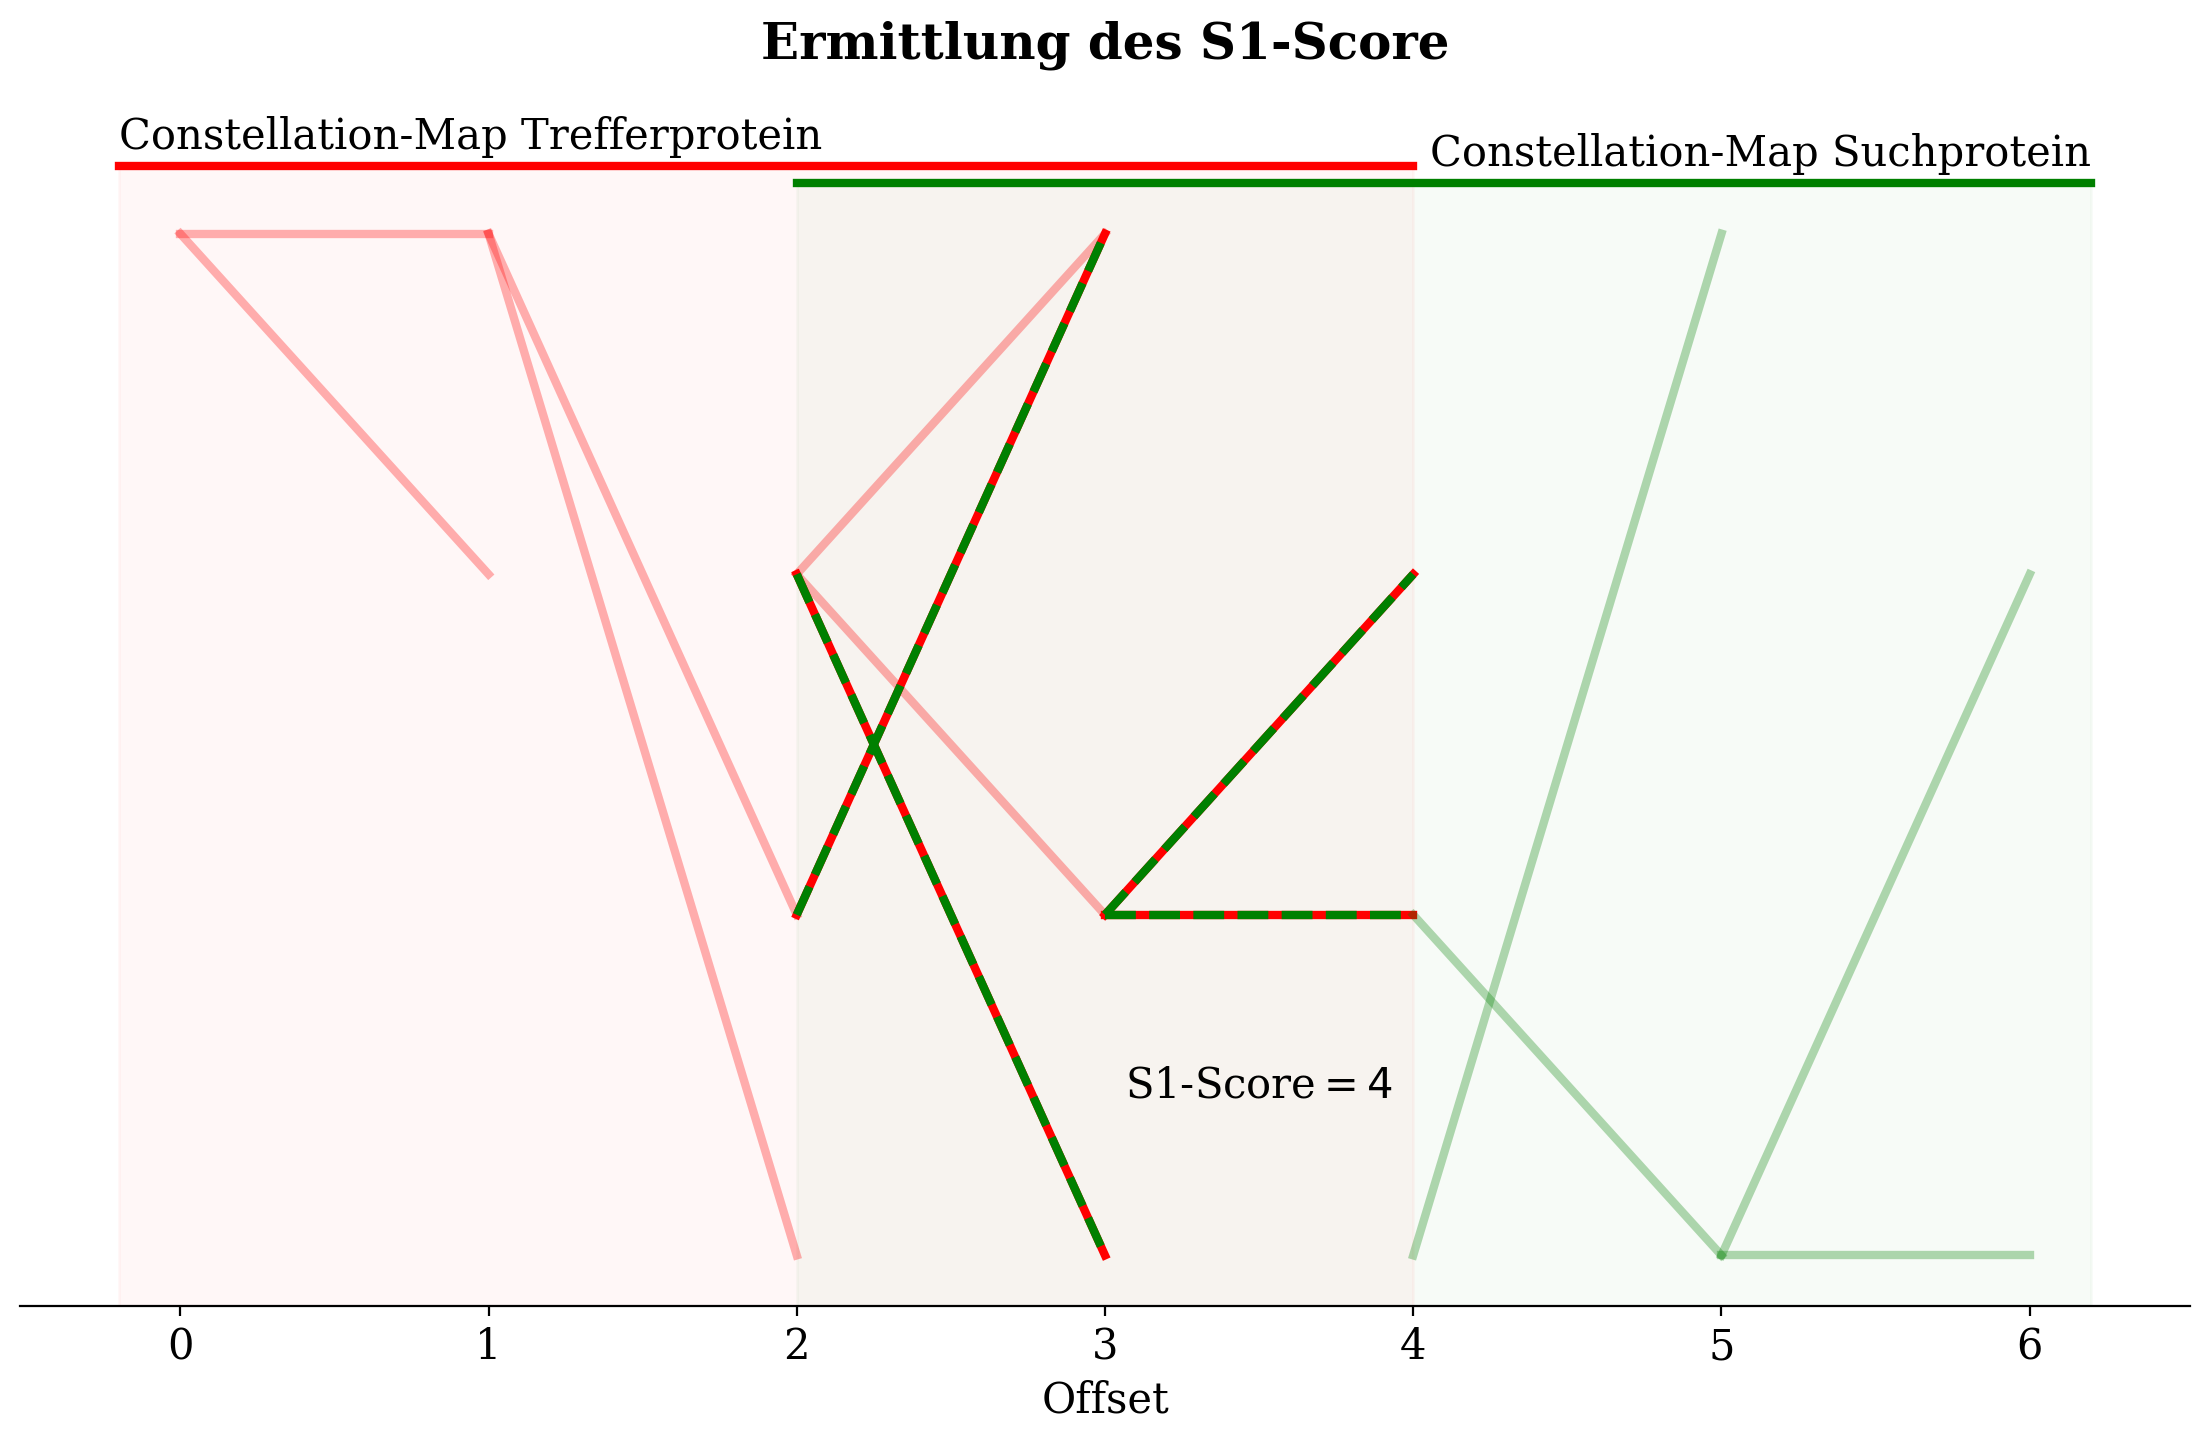
\includegraphics[width=\Width]{plot_scoring.png}
                    \caption[Ermittlung des S1-Score]{Die Constellation-Maps werden aneinander verschoben. Die maximale Überschneidung bei Offset 2 ist der Score. Hier stimmen 4 Hashes in Position überein, sie liegen genau übereinander und sind somit gestrichelt dargestellt.}
                    \label{fig:scoring}
                \end{figure}
                \end{minipage}

                Da große Proteine mit sehr langen Aminosäuresequenzen kürzere Sequenzen kleinerer funktionsungleicher Proteine enthalten können, reicht der ermittelte Score alleine nicht aus, da in diesem Fall sehr viele Kanten der Eingabe-\ac{CM} übereinstimmen würden, sodass trotz Mis-Match der nahezu maximale Score erreicht werden würde. Bezogen auf das Beispiel zu S1 in \autoref{fig:scoring}, wäre dort der grüne Bereich vollständig vom roten Bereich eingeschlossen mit Überschneidungen in beinahe allen Kanten.

                Um das zu umgehen, wird der \ac{JSI} verwendet, einem Maß, das die Übereinstimmung zweier Mengen A und B wie folgt bewertet:
                \begin{equation}
                    \label{equ:jsi}
                    JSI(A, B)=\frac{|A \cap B|}{|A \cup B|}
                \end{equation}
                Dieser Index nimmt einen Wert von 0 an, wenn beide Mengen disjunkt sind, und nähert sich der 1 je größer die Schnittmenge ist. Im Fall des Vergleichs zweier Constellation-Maps, also zwei Hash-Mengen, wird hier bewertet, wie viele Kanten sich die beiden Maps positionsunabhängig teilen. Durch diese Unabhängigkeit reicht der JSI alleine nicht als Score aus, sodass nur in Kombination/Multiplikation mit dem S1 ein robuster Score entsteht, da beide zusammen ihre Schwächen aufheben. Der \ac{JSI} in \autoref{fig:scoring} beträgt $\frac{4}{14} \approx 0.286$, da die Schnittmenge beider Hashmengen hier gleichzeitig den S1-Score bilden und die restlichen Hashes disjunkt zueinander sind. Der S1 wäre nur noch 3, wenn eine der markierten Kanten an einer anderen Position wäre, wobei der \ac{JSI} davon unberührt bliebe.

            \item \PhantomSubSub[fam.matching]{Family-Matching}
                \textbf{Family-Matching:}\ \ Eingabe ist eine \ac{CSV}-Tabelle mit der Zuordnung von Protein-ID und -familie (mittels Familien-ID). Die für das Matching verwendeten Hashes sind hier diejenigen, die sich alle Mitglieder einer Suchfamilie teilen. Die Idee dahinter ist, dass diese Hashes spezifisch für diese Familie, beziehungsweise deren Funktion ist. Als Bewertungsmaß wird dabei die Anzahl Hashes des Treffers verwendet, die mit den Familienhashes übereinstimmen. Der Vorteil dieses Ansatzes ist, dass durch die Reduktion der betrachteten Hashes die Laufzeit im Vergleich zum Single-Protein-Matching verringert wird. Denn für jeden Hash muss in der Datenbank durch alle Proteine iteriert werden, die ebenfalls diesen Hash haben. Je weniger Hashes also betrachtet werden, desto weniger Iterationen gibt es. Da die geteilten Hashes einer Familie in der Anzahl nur kleiner oder gleich der Anzahl Hashes des Familienmitglieds mit den wenigsten Hashes sein können, ist dieser Ansatz somit mindestens so schnell wie für das Single-Protein-Matching mit diesem kleinsten Mitglied.

                Für die Ausgabe werden diese Treffer zusammengefasst. Dazu gibt es zwei Kriterien, den F-Score und die Schärfe (Sharpness), die nach folgender Berechnung ermittelt werden:
                \begin{equation}
                    \label{equ:f_score}
                    \begin{split}
                        t & = \texttt{max\_score}(TrP)\\
                        Sharpness & = \begin{cases}
                                          \frac{t-\texttt{max\_score}(FP)}{t},& \text{if t} > 0\\
                                          \sminus 1,& \text{sonst}
                                      \end{cases}\\
                        Precision & = \frac{|TrP|}{|TrP|+|FP|}\\
                        Recall & = \frac{|TrP|}{|TrP|-member\_count}\\
                        F\_Score & = \frac{2 \cdot Precision \cdot Recall}{Precision + Recall}
                    \end{split}
                \end{equation}

                TrP ist hierbei die Menge der Treffer, die tatsächlich in der Familie vorkommen (true positives), wobei FP diejenigen sind, die das nicht tun (false positives) und einen besseren Score als der letzte korrekte Treffer haben. ``member\_count'' ist die Anzahl an Mitgliedern der Familie.

                Die Schärfe stellt das Verhältnis der besten Scores von FP und TrP dar, also wie weit der beste korrekte Treffer im Score von dem besten falschen Treffer entfernt ist.

                Die Präzision gibt an, wie viele der Treffer korrekt gewesen sind, während der Recall zeigt, wie viele der Familienmitglieder gefunden wurden. Der F-Score bringt diese beiden Werte zusammen.

                Die Ausgabe von \protfin\ Version 0.4 als \ac{CSV}-Tabelle beinhaltet aktuell diese Zusammenfassung zu Entwicklungszwecken. Sollte \protfin\ ausgereift sein, wird die Ausgabe vermutlich die Treffer je Suchfamilie enthalten. In den Spalten wird folgendes dokumentiert:
                \begin{enumerate}[1.]
                    \item Family\_ID $\rightarrow$ ID der Suchfamilie
                    \item F\_Score
                    \item Precision
                    \item Recall
                    \item Sharpness 
                    \item Member\_Count $\rightarrow$ Anzahl der Mitglieder der Suchfamilie
                    \item Match\_Count $\rightarrow$ Anzahl gefundener Treffer
                    \item Hash\_Intersec\_Size $\rightarrow$ Anzahl der Hashes, die sich die Mitglieder teilen
                \end{enumerate}
        \end{enumerate}

    % subsection grundalgorithmus (end)
    \begin{experiment}{UniRef90 Sampling} % (fold)
        \label{exp:uniref90}
        Ein Bestandteil der Strukturanalyse in \autoref{alg:strukturdaten} ist die Selektion signifikanter Frequenzen zur Erstellung der \ac{CM}. Es wäre zwar möglich, alle Frequenzen auszuwählen und dafür die Signalstärke in den Hash einfließen zu lassen, jedoch führe diese Vorgehensweise zu wesentlich mehr Hashes und einer folglich sehr großen Datenbank, was wiederum das Scoring/Matching verlangsamt. Ein Anspruch an \protfin\ ist, dass die Datenbankgröße die Eingabegröße nicht wesentlich übersteigt, wobei es sich bei der Eingabe um eine einfache FASTA-Datei handelt.

        Diesem Problem soll durch ein Sampling-Experiment abgeholfen werden. Darin wurden aus etwa 180 Millionen Sequenzen der UniRef90 Datenbank je ein zufälliges Fenster fester Größe für die \ac{STFT} ausgewählt, transformiert und die Signalstärken je Frequenz gemerkt. Um daraus eine Selektionsmethode abzuleiten, wurden die Grenzquantile einer jeden Frequenz ermittelt, um signifikant seltene Signalstärken zu ermitteln. Folglich war es möglich, für die Constellation-Map nur diejenigen Frequenzen zu behalten, welche in den Randzonen der Signalstärken liegen, sodass nicht nur Signale infrage kommen, die für eine besonders starke Ausprägung eines Kidera-Faktors sprechen, sondern auch für den Fall der umgekehrten Ausprägung, wie z.B. Hydrophilie statt Hydrophobie.

        \autoref{alg:strukturdaten} wurde daher anschließend insofern angepasst, dass bei der Frequenz-Selektion in \autoref{alg:strukturdaten:selection} die gewählten Frequenzen so ermittelt werden, dass je Grenzwert die Ausreißer ausgewählt werden, also einmal für den oberen Wert und dann für den unteren Wert, und aus diesen Ausreißermengen die Maxima selektiert werden. Zudem wird einem Hash je Frequenz noch mit einem Bit die Information hinzugefügt, ob die Amplitude besonders hoch oder niedrig ist.

        Die zu klärende Frage war, welche Grenzquantile verwendet werden müssen, um eine möglichst gute Frequenzauswahl zu erzielen, für ein gutes Matching mit kleineren Datenbanken.
    \end{experiment}
    \begin{experiment}{Filter Hashes} % (fold)
        \label{exp:filter_hashes}
        Die Experimente zu vorigen Versionen von \protfin\ haben zu sehr großen Datenbanken und entsprechend langsamem Matching geführt. Mit dem Ziel, die Datenbank auf Eingabegröße zu reduzieren, sollte darin je Protein nur das Notwendigste gespeichert werden. In \autoref{exp:uniref90} wurde dafür die Frequenzwahl angegangen, indem die Grenzwerte mit der Wahl der Maxima kombiniert wurden. Alternativ soll hier die Größe durch einen Filter ermöglicht werden, wobei die Grenzwerte als alleiniges Selektionskriterium dienen. Zum Filtern wurden dazu nach der Datenbankerstellung nur die Einträge der quantilsmäßig seltensten Hashes behalten. Die entfernten Hashes an sich wurden zudem in einer Blacklist gespeichert, um sie vor dem Matching auch aus den Hashes der Suchsequenzen zu entfernen, da sie ansonsten den \ac{JSI} verfälschen würden, weil entfernte Hashes nicht in der Schnittmenge auftauchen könnten.

        Auch in diesem Experiment musste herausgefunden werden, welches Quantil sich am besten eignet. Je kleiner es ist, desto kleiner wird auch die Datenbank, aber umso ungenauer auch das Matching. Es galt einen guten Kompromiss zu finden.
    \end{experiment}
    \begin{experiment}{\acl{TZ}} % (fold)
        \label{exp:target_zone}
        Die \ac{TZ} beschreibt in \autoref{fig:hashing} die maximal mögliche Kantenlänge eines Hashes, also die Anzahl Nachfolgefenster, die für das Hashing herangezogen werden. Je größer die \ac{TZ}, desto näher kommt die Constellation-Map einem vollständigen Graphen, was die Datenbankgröße entscheidend beeinflusst. Da die \ac{TZ} mit 12 Bit (\autoref{fig:hash}), also 4096, für Aminosäuresequenzen nahezu unbeschränkt ist, wurde in diesem Experiment geprüft, wie wenige Bits ausreichen, um noch ein gutes Matching zu gewährleisten. Umgesetzt wurde dies in \RefAlgLine{alg:hashing}{target_zone}, wo über die Nachfolger iteriert wurde. Um die \ac{TZ} einzubeziehen, wurden die hard-coded $2^{12} - 1$ mit einer zusätzlichen Variable zu $2^{targetZoneBits} - 1$ erweitert. Als Selektiosmethode wurd der Ansatz aus \autoref{exp:uniref90} verwendet.
    \end{experiment}
    \begin{experiment}{Selection-Method} % (fold)
        \label{exp:selection_method}
        Dieses letzte Experiment knüpft an \autoref{exp:uniref90} an. Dort war die Intention, die ermittelten Grenzwerte mit einer anschließenden Maxima-Wahl zu kombinieren. Hier wurden nun folgende Ansätze versucht:
    
        \begin{enumerate}
            \item Es werden alle Frequenzen ausgewählt, deren Amplituden den oberen/unteren Grenzwert aus \autoref{exp:uniref90} über-/unterschreiten. Es bilden also die Grenzwerte allein die Selektionsbedingung.
            \item Es werden erst Frequenzen über Maxima ausgewählt und anschließend aus diesen nur diejenigen behalten, die den oberen Grenzwert überschreiten. Gleiches wird für Minima mit dem unteren Grenzwert wiederholt.
            \item Die Amplituden der Frequenzen werden in ihren Abstand zum oberen Grenzwert umgerechnet. Für jede Frequenz wurde in \autoref{exp:uniref90} zudem die Standardabweichung der gesampelten Amplituden ermittelt. Die Abstände werden durch die Division dadurch normalisiert. In diesen normalisierten Abständen werden die Frequenzen nach lokalen Maxima ausgewählt und nur die behalten, die den oberen Grenzwert überschreiten. Das ganze Verfahren wird für den unteren Grenzwert mit lokalen Minima wiederholt.
        \end{enumerate}

        Diesen beiden Methoden wurden zusätzlich durch einen Parameter $k$ erweitert, welcher bestimmt, dass die ersten $k$ Frequenzen im Nachhinein aus der Auswahl entfernt werden (entsprechend ihrer Reihenfolge wie im Beispiel in \autoref{fig:freq_selection}, also $k=2$ entfernt Frequenzen 0,1). Das hatte den Hintergrund, dass in niedrige Frequenzen in  oft ausgewählt wurden.

        Die vorigen Ergebnisse hatten zudem veranlasst, das Signifikanzniveau der gesampelten Amplituden von 5\% zu verringern, sodass zusätzlich die Grenzwerte für $\alpha \in \{0.1\%, 0.01\%, 0.001\%\}$ ermittelt werden sollten. Aufgrund eines Rechenfehlers wurden tatsächlich die Werte für $\alpha \in \{10\%, 1\%, 0.1\%\}$ berechnet, was bis zum Verfassen dieser Arbeit unentdeckt blieb. Als Obergrenze wurde immer der maximale Amplitudenwert verwendet. Um die Laufzeit dieses Experiments durch zu viele Parameterwerte nicht unnötig zu erhöhen, wurden vor der Durchführung die pro \ac{TP} selektierten Frequenzen gezählt und die mittlere Anzahl Frequenzen pro Fenster ermittelt, um die zu testenden $\alpha$-Werte zu begrenzen.

        Um die Ansätze effizient zu testen, wird für dieses Experiment die Datenbankerstellung in \autoref{alg:datenbank} so angepasst, dass sie abgebrochen wird, sobald der Speicherbedarf das 6-fache der Eingabedaten übersteigt. Wenn eine Datenbank nicht größer als die Eingabe sein soll, dürfen die Daten einer Sequenz nicht den Speicherbedarf der Textrepräsentation ihrer Aminosäuren überschreiten. Diese Zeichen sind Teil des \ac{ASCII} und benötigen daher nur 1 Byte Speicher, was bedeutet, dass bei einer Sequenz der \ac{TP} mit einer medialen Länge von etwa 300 Aminosäuren nur ebensoviele Bytes verwendet werden dürften. Hierzu eine Rechnung unter der Annahme, es gäbe nur eine Frequenz pro Fenster:
        \begin{equation}
            \begin{split}
                target\_zone &= 8\\
                \emph{fenster\_größe} &= 30\\
                \emph{überlappung} &= 15\\
                \emph{sequenz\_länge} &= 300\\
                anzahl\_fenster &= \frac{\emph{sequenz\_länge}}{\emph{fenster\_größe} - \emph{überlappung}} = 20\\
                \emph{hash\_größe} &= 32\ Bit = 4\ Byte\\
                speicher\_pro\_kf &= target\_zone \cdot anzahl\_fenster \cdot \emph{hash\_größe} = 640\ Byte\\
                anzahl\_kf = 10\\
                datenbank\_speicher &= target\_zone \cdot anzahl\_fenster \cdot \emph{hash\_größe} \cdot 10 = 6400\ Byte
            \end{split}
        \end{equation}

        Selbst bei einer Frequenz pro Fenster wäre die Datenbank nach dieser Abschätzung doppelt so groß wie die Eingabe. Dieses Kriterium floss bei der Auswahl der $\alpha$-Werte für dieses Experiment ein.
    \end{experiment}
    \subsection{Durchführung} % (fold)
        \label{sub:durchführung}
        Die Durchführung der Experimente läuft nach einem immergleichen Schema ab. Zuerst werden mit den MapMan-Referenz-Proteinen aus \autoref{sub:mapman} die Datenbanken erstellt und anschließend mit einer Teilmenge dieser Proteine das Single-Protein-Matching durchgeführt. Diese Teilmenge wird über die MapMan-Bins ausgewählt. Um die Suchproteine nämlich möglichst funktional divers zu halten, werden je Wurzelknoten der Bins sieben zufällige Sequenzen ausgewählt. Für das Family-Matching werden alle die MapMan-Bins mit ihren Proteinen einbezogen, die durch mehr als einem Protein verteten werden.

        Neben den experimentspezifischen Parametern, wie Quantilen oder der Größe der \acl{TZ}, werden zusätzlich jedes Mal Parameter getestet, die die \ac{STFT} und somit alle Experimente betreffen, da sich die Werte dazu aufgrund der zu digitaler Musik vergleichsweise kurzen Sequenzen nicht direkt von SHAZAM ableiten lassen. Hierbei geht es um die \ac{FG}, die Länge der Überlappung zwischen benachbarten Fenstern und $n\_peaks$, der Anzahl Frequenzen, die von den ausgewählten signifikanten Frequenzen verwendet werden. Werden also $n+x$ Frequenzen ausgewählt, werden die $x$ am wenigsten signifikanten Frequenzen entfernt, im Gegensatz zu $k$ aus \autoref{exp:selection_method}, welches unabhängig der Anzahl immer dieselben Frequenzen entfernt. Alle Parameter mit ihren getesteten Werten sind in \autoref{tab:parameter} aufgelistet:
        
        \begin{table}[H]
            \centering
            \caption{Experiment-Parameter}
            \label{tab:parameter}
            \begin{minipage}{\textwidth}
                Bei dem Parameter Quantil handelt es sich um das Quantil der Hashes, das beim Filtern der Datenbank behalten wird (siehe \autoref{exp:filter_hashes}). Die Signifikanz bezeichnet das Signifikanzniveau $\alpha$, welches in \autoref{exp:uniref90} verwendet wird, um aus den Fenster-Samples die Grenzwerte für auffällige Amplituden einer Frequenz zu bestimmen. Für das Matching wird bei \autoref{exp:uniref90} lediglich $\alpha=5\%$ betrachtet.
            \end{minipage}
            \begin{tabular}{lllllll}
            \toprule
             \textbf{Parameter} & \multicolumn{5}{l}{\textbf{Werte}} & \textbf{Experimente}\\
             \midrule
             \acf{FG}    & 10 & 20    & 30     & 40     & 50        &~\ref{exp:uniref90},~\ref{exp:target_zone}\\
                         &    & 20    & 30     & 40     & 50        &~\ref{exp:filter_hashes}\\
                         &    &       & 30     & 40     & 50        &~\ref{exp:selection_method}\\
             $n\_peaks$  &alle& 3     & 5      &        &           &~\ref{exp:uniref90},~\ref{exp:target_zone},~\ref{exp:selection_method}\\
                         &    & 3     & 5      &        &           &~\ref{exp:filter_hashes}\\
             Overlap     & 0  & 25\%  & 50\%   & 75\%   &$\ac{FG}-1$&~\ref{exp:uniref90},~\ref{exp:filter_hashes},~\ref{exp:target_zone}\\
                         &    & 25\%  & 50\%   & 75\%   &           &~\ref{exp:selection_method}\\
             \acl{TZ}    & 8  & 16    & 32     & 64     &           &~\ref{exp:target_zone}\\
                         & 8  &       &        &        &           &~\ref{exp:selection_method}\\
             Quantil     &0.1 & 0.2   & \dots  & 0.9    &     1     &~\ref{exp:filter_hashes}\\
             Signifikanz &5\% & 10\%  &   1\%  & 0.1\%  &           &~\ref{exp:uniref90}\\
                         &    &       &   1\%  & 0.1\%  &           &~\ref{exp:selection_method}\\
                         &5\% &       &        &        &           &~\ref{exp:filter_hashes},~\ref{exp:target_zone}\\
             \bottomrule
            \end{tabular}
        \end{table}
    % subsection durchführung (end)
% section methoden (end)
